\subsection{Performance}
\label{sec:performance}
This section evaluates the performance of the driver and shows the impact on the \emph{Google Chrome} browser. At first, the impact on \emph{Chrome} is measured. Then, the time needed for hashing a \gls{DLL} file is measured.

\subsubsection{Hardware}
The performance measurement was done in a \emph{VirtualBox}\footnote{\url{https://www.virtualbox.org/}} virtual machine running \emph{Windows 7 64 bit}. Table \ref{fig:hardware_host} shows the hardware used for the host computer. Table~\ref{fig:hardware_vm} shows the hardware assigned to the virtual machine. The virtual machine was stored on a RAID 1 setup with 50 GB of assigned storage. 
\begin{table}
\centering
\caption{Hardware of the host system}
\label{fig:hardware_host}
\begin{tabularx}{\textwidth}{|l|X|}
\hline
Component & Used Hardware \\ \hline
CPU & Intel i7-2600k @ 3.5 GHz, 4 cores, 8 threads \\ \hline
RAM & 4 * 4 GB @ 1600 MHz \\ \hline
MAINBOARD & Asus P8Z68 deluxe/gen3 \\ \hline
SSD 1 & Mushkin Chronos 120 GB, 500 MB/s \\ \hline
SSD 2 & San Disk Pro 480 GB, 500 MB/s \\ \hline
RAID 1 & 2x Western Digital Caviar Green 2.5 TB, 170 MB/s \\ \hline
\end{tabularx}
\end{table}
\begin{table}
\centering
\caption{Assigned hardware of the virtual machine}
\label{fig:hardware_vm}
\begin{tabularx}{\textwidth}{|l|X|}
\hline
Component & Used Hardware \\ \hline
CPU & Intel i7-2600k @ 3.5 GHz, 1 core, 2 threads \\ \hline
RAM & 4 GB @ 1600 MHz \\ \hline
\end{tabularx}
\end{table}

\subsubsection{General setup}
The experiments used \emph{Google Chrome} version \emph{48.0.2564.97 m} and disabled several services of the \emph{Windows} operating system to get more accurate test results. \emph{Windows Defender}, \emph{Windows Search} and \emph{Windows Update} were disabled for both, host and guest machine. Every test was executed ten times for each possible configuration.

\subsubsection{Experiment 1}
In Experiment 1 the performance impact of the implemented driver on Google Chrome is measured. The internal structure of the driver was used to create the four main groups of measurement, without the driver, with the \gls{WPM} component, with the \gls{DLL} load component and with both components. This test was then done for 1, 2, 4, 8 and 16 opened tabs and data was obtained for a duration of 1, 2, 4, 8 and 16 minutes of runtime. The measurement was done with Google Chrome's internal profiler\footnote{\url{chrome://profiler}}. In total this results in 200 data files obtained through the profiler which was then used to evaluate the performance decrease. The resulting 200 data files are merged with five different operations, minimum, maximum, median, mean and sum of all values. The titles of the resulting plots have been abbreviated to their respective function names of Section \ref{sec:profiler}. Considering the implementation of the driver, this experiment should show that the execution without the driver is faster.
\begin{figure}[!htbp]
	\centering
    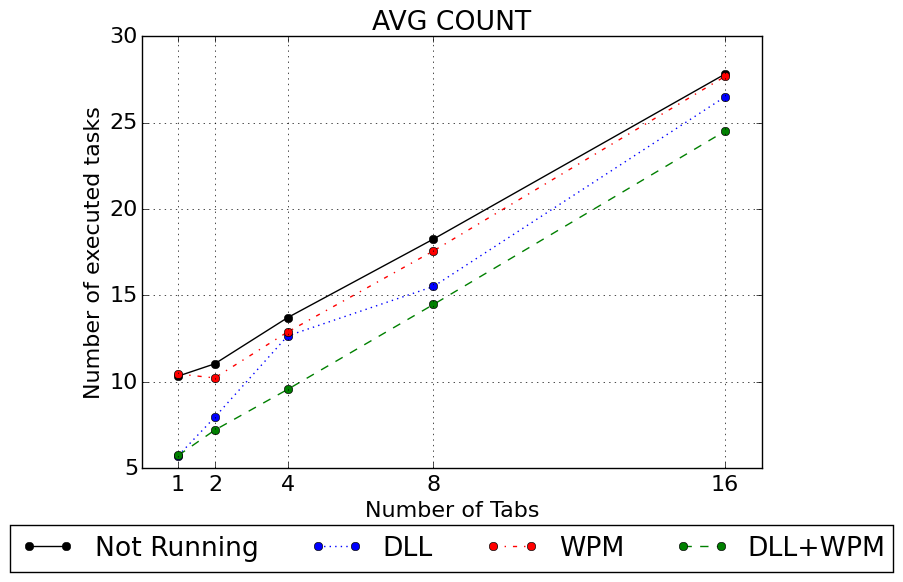
\includegraphics[width=\textwidth,height=0.45\textheight,keepaspectratio]{Evaluation/experiment1/AVG-COUNT-2.png}
    \caption{Average count, 2 minutes of data}
    \label{fig:ex1_avgcount_2}

  	\vspace*{\floatsep}
  	
    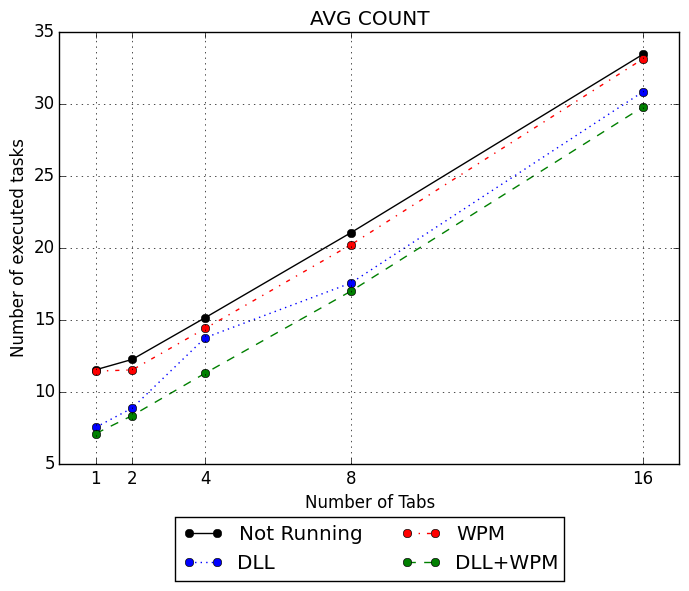
\includegraphics[width=\textwidth,height=0.45\textheight,keepaspectratio]{Evaluation/experiment1/AVG-COUNT-16.png}
    \caption{Average count, 16 minutes of data}
    \label{fig:ex1_avgcount_16}
\end{figure}
Figure \ref{fig:ex1_avgcount_2} shows the average count of tasks that were executed over two minutes. Running both components, \emph{\gls{DLL}+\gls{WPM}} is the slowest of all four configurations, because the average number of executed tasks is the lowest. \emph{WPM} and the \emph{Not Running} are almost equal with \emph{\gls{WPM}} being one task slower in for two and fours tabs. Figure \ref{fig:ex1_avgcount_16} shows the same measurement for a duration of 16 minutes. The result is the same as of Figure \ref{fig:ex1_avgcount_2}. The comparison between both plots show that there is not much of a difference between a one and 16 minute measurement, but the 16 minute measurements give more accurate results. What is more interesting about these graphs is the linear trend of the four plots. For each added tab only about 1.5 times more tasks are executed. This is consistent throughout all four plots.
\begin{figure}[!htbp]
	\centering
    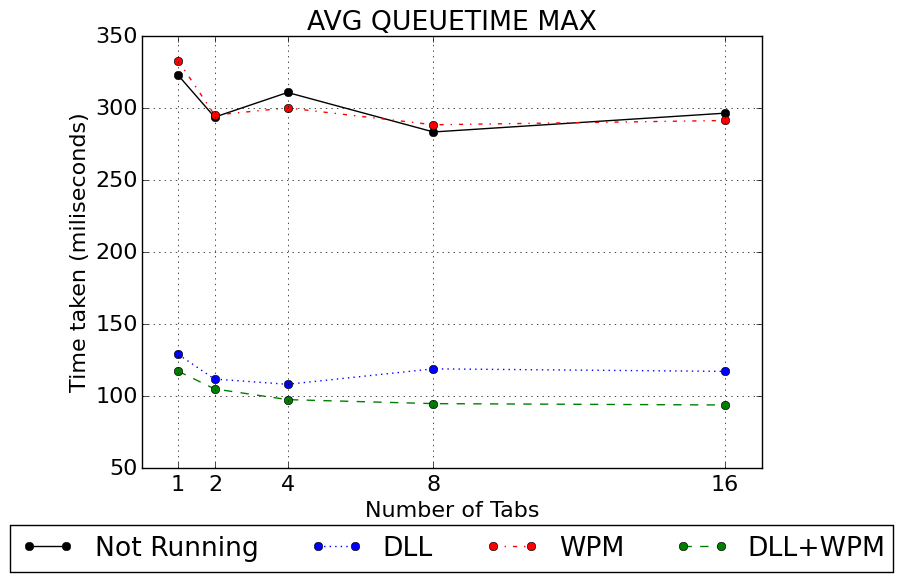
\includegraphics[width=\textwidth,height=0.45\textheight,keepaspectratio]{Evaluation/experiment1/AVG-QUEUETIME-MAX-1.png}
    \caption{Average of the maximum queuetime, 1 minute of data}
    \label{fig:ex1_avgqueuetimemax_1}

	\vspace*{\floatsep}

    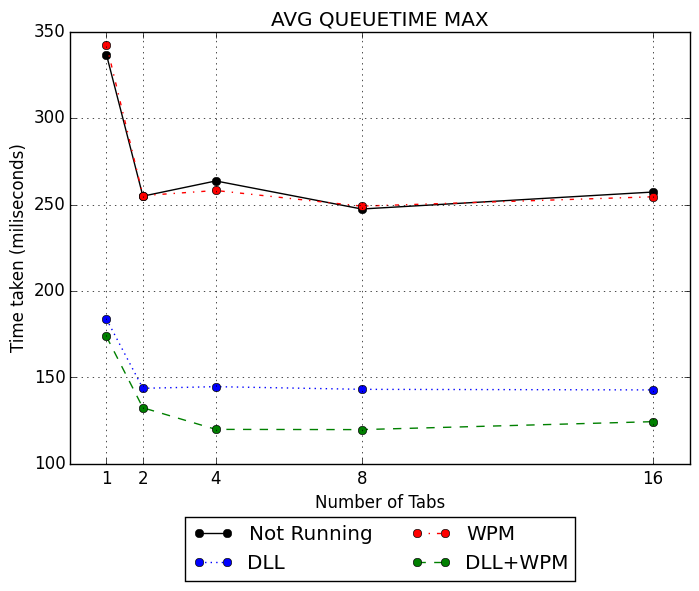
\includegraphics[width=\textwidth,height=0.45\textheight,keepaspectratio]{Evaluation/experiment1/AVG-QUEUETIME-MAX-16.png}
    \caption{Average of the maximum queuetime, 16 minutes of data}
    \label{fig:ex1_avgqueuetimemax_16}
\end{figure}
This property of Chrome being faster (executing more task) without a driver running can be seen too in the next two Figures \ref{fig:ex1_avgqueuetimemax_1} and \ref{fig:ex1_avgqueuetimemax_16}. These graphs show the average of the maximum queuetime. The y-axis shows the average number of milliseconds a task was waiting for execution. Again, two groups form, \emph{Not Running} with \emph{\gls{WPM}} and \emph{\gls{DLL}} and \emph{\gls{DLL}+\gls{WPM}}. Tasks without running driver queue in average longer than tasks with running driver. The reason for that is \emph{Not running} executes more tasks, which leads to some tasks queuing longer because Chrome is busy with running other tasks. Accordingly, the average queuetime for the \gls{DLL} component and both components running is lower, because less tasks are executed and Chrome is less busy with task execution. The overhead of the driver is clearly present in the figures and tasks are in average waiting 100 milliseconds less than without running the driver. This means, that the average overhead per task introduced to the driver is 100 milliseconds for the queuetime.
\begin{figure}[!htbp]
	\centering
    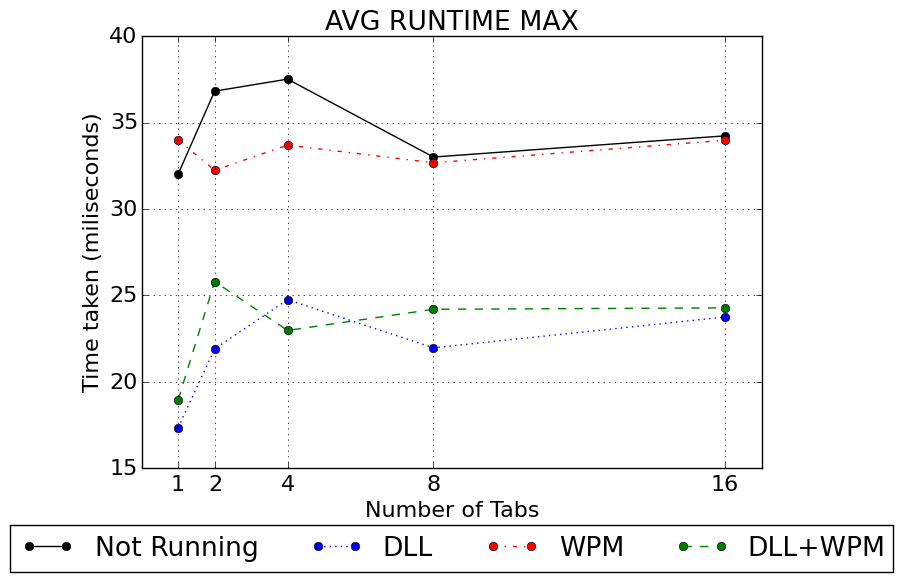
\includegraphics[width=\textwidth,height=0.45\textheight,keepaspectratio]{Evaluation/experiment1/AVG-RUNTIME-MAX-1.png}
    \caption{Average of the maximum runtime, 1 minute of data}
    \label{fig:ex1_avgruntimemax_1}
    
  	\vspace*{\floatsep}    
    
    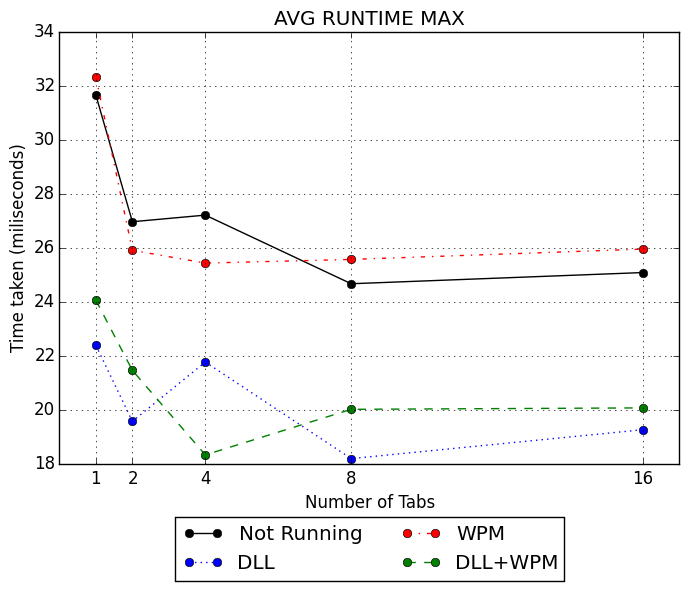
\includegraphics[width=\textwidth,height=0.45\textheight,keepaspectratio]{Evaluation/experiment1/AVG-RUNTIME-MAX-16.png}
    \caption{Average of the maximum runtime, 16 minutes of data}
    \label{fig:ex1_avgruntimemax_16}
\end{figure}
Figure \ref{fig:ex1_avgruntimemax_1} and Figure \ref{fig:ex1_avgruntimemax_16} show the average of the maximum runtime of all tasks for one and 16 minutes. The results of this plots are similar to Figure \ref{fig:ex1_avgqueuetimemax_1} and Figure \ref{fig:ex1_avgqueuetimemax_16}. The average runtime of \emph{Not Running} and \emph{\gls{WPM}} is higher than \emph{\gls{DLL}} and \emph{\gls{DLL}+\gls{WPM}}. This is again a result of the higher number of tasks executed and Chrome being already busy executing other tasks. Additionally, tasks are waiting for other tasks to be finished with execution, extending the runtime.
\begin{figure}[!htbp]
	\centering
    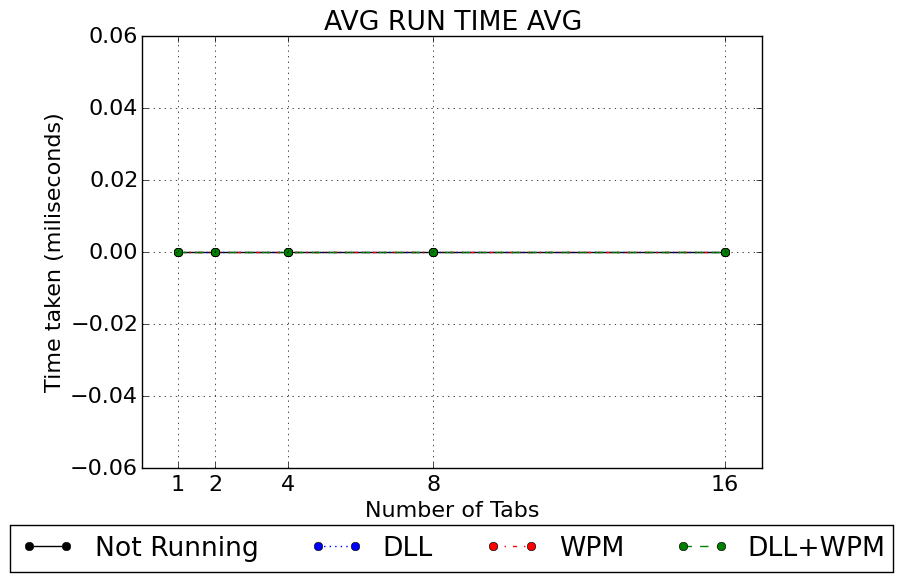
\includegraphics[width=\textwidth,height=0.45\textheight,keepaspectratio]{Evaluation/experiment1/AVG-RUNTIME-AVG-1.png}
    \caption{Average of the average runtime, 1 minute of data}
    \label{fig:ex1_avgruntimeavg_1}
    
  	\vspace*{\floatsep}    
    
    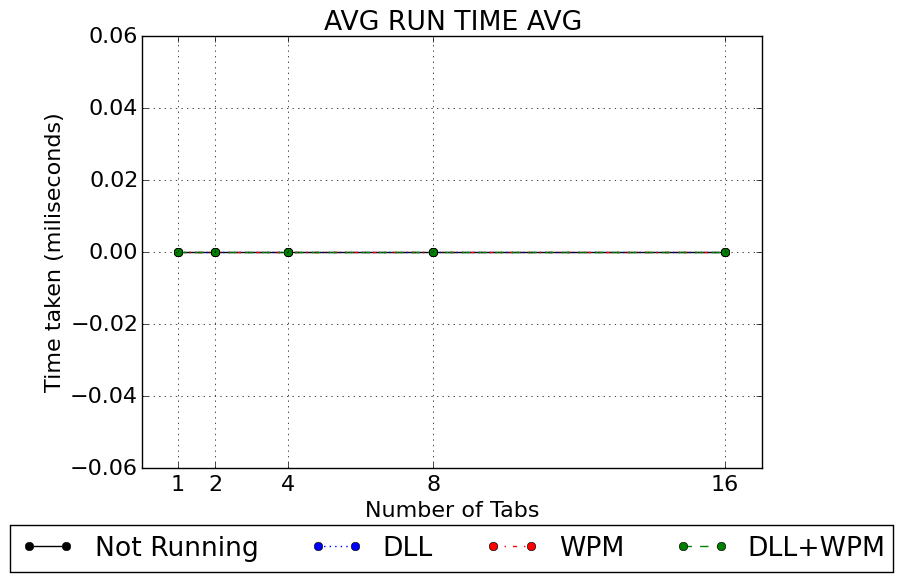
\includegraphics[width=\textwidth,height=0.45\textheight,keepaspectratio]{Evaluation/experiment1/AVG-RUNTIME-AVG-16.png}
    \caption{Average of the average runtime, 16 minutes of data}
    \label{fig:ex1_avgruntimeavg_16}
\end{figure}
At the end of this experiment, a look is taken at the average of the average runtime of a task. This data is shown in Figure \ref{fig:ex1_avgruntimeavg_1} for one minute and Figure \ref{fig:ex1_avgruntimeavg_16} for 16 minutes. The result is, that there is in average no difference between running the driver and not running it. For both Figures, the average runtimes are zero. This means, because the runtimes are using rounded values, the execution took less than 0.50 milliseconds in average.

\medskip

The result of this experiment 1 is, that the driver slows down execution during startup, which increase maximum run- and queuetime. There is no difference during the later usage, as the average of the average runtimes are staying constant. The reason for this performance decrease can be found in the \gls{DLL} component of the driver, as the other one, the \gls{WPM} component is running with almost no performance decrease. The \gls{DLL} component will be evaluated further in experiment 2.
\clearpage
\subsubsection{Experiment 2}
\begin{figure}[h]
	\centering
    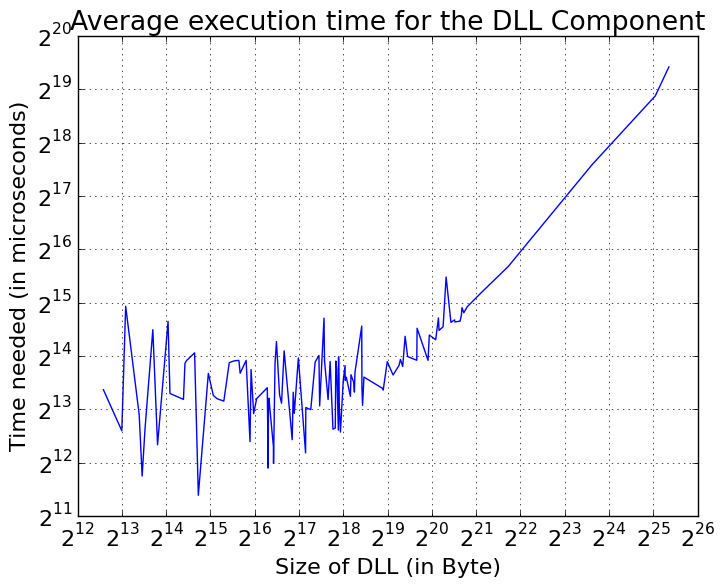
\includegraphics[width=\textwidth,height=0.45\textheight,keepaspectratio]{Evaluation/experiment2/result.png}
    \caption{Average execution time for sha256 file hashing}
    \label{fig:ex2_result}
\end{figure}
In Experiment 2 the performance impact of the \gls{DLL} component is evaluated. Experiment 2 uses the same hardware and software setup as Experiment 1. As the result of Experiment 1 showed, that running the \gls{DLL} component slowed down the execution of \emph{Google Chrome}, Experiment 2 tries to find the actual reason for that result. Looking at the code, and running time measurements on it leads to the sha256 file hashing slowing down the execution. Figure~\ref{fig:ex2_result} shows the average of ten independent measurements. For file sizes between four kilobyte ($2^{12}$ byte) and one megabyte ($2^{20}$ byte), the needed time is roughly constant around 16 milliseconds ($2^{14}$ microseconds). Increasing the file size further than one megabyte results into increase of time for hashing the file. The graph uses logarithmic scaling with base two one both axis, which give a better comparability of the actual result. Starting at one megabyte, doubling the file size will double the necessary time to create the sha256 hash. Most \glspl{DLL} are rather small (less than one megabyte) and will require constant time for file hashing. However, in contrast to that, some are very large (around 50 megabyte or even larger) and will require with respect to the given file size linearly more time. An example for that can be found in \emph{Google Chrome's} used \glspl{DLL}. \emph{Chrome\_child.dll} with 40 megabyte and \emph{chrome.dll} with 30 megabyte make up most of the time that is spent for hashing during \emph{Chrome's} process creation. As the initial callback function \syscall{PsSetLoadImageNotifyRoutine} is acting synchronous, so is the hashing of files. Therefore, the process is suspended for the whole time that is needed for hashing all \glspl{DLL}. A single process creation is delayed by the sum of the required time for hashing all \glspl{DLL}, which makes up a total of 2905253 microseconds, or 2.9 seconds.

\paragraph{Impact of \gls{DLL} injections}
In case of an actual attack with \gls{DLL} injections, it is interesting to know which performance impact is present for \emph{Google Chrome}. According to Experiment 2, the time required for hashing is
\begin{equation}
t(x) = \min\{2^{14} * 2^{\log_2(x) - 20}, 2^{14}\} \label{eq:one}
\end{equation}
where $x$ is the file size in bytes of the \gls{DLL} and $t(x)$ is the required time in microseconds for calculating the hash. The time cost of (\ref{eq:one}) is scaling linearly with the size $x$ of the \gls{DLL} file. Therefore, especially for larger files it is interesting to know if hashing is required every time the \gls{DLL} is mapped into memory. In the current implementation, hashing occurs only once, if the \gls{DLL} is not on the whitelist. This is due to \emph{Windows} internal \gls{DLL} loading behavior. The result of patching a \gls{DLL} is an invalid executable format. As soon as a second \gls{DLL} load request for the same file is done, the \emph{Windows} kernel will return early with error \syscall{ERROR\_BAD\_EXE\_FORMAT}. This behavior will stay until the file is unloaded from memory which will happen when exiting \emph{Chrome}. In the other case, where the \gls{DLL} is in the whitelist, there is no such way of returning early. The \gls{DLL} file will need to be hashed again if it is not present in the process virtual memory. This is another limitation of the approach using \syscall{PsSetLoadImageNotifyRoutine}.
\clearpage
